%===================================== CHAP 4 =================================

\chapter{Results and Analysis}
\label{chap:results}
Results are presented in the following chapter. The chapter is separated into sections in line with the categories defined in section~\ref{subsec:data-req}, in the following order: miscellaneous, research transparency, method documentation, experiment documentation,  and open data. At the end a section on researcher error is included.

\section{Miscellaneous}
Variables in the miscellaneous category describe the research and include the following variables: affiliation, conference, research type, result outcome, and third-party citation.
The data for each variable except conference can be seen in figure~\ref{fig:miscellaneous-data}. The conference distribution is seen in table~\ref{tab:conferences}.

Note that the Third-party citation data in figure~\ref{fig:third-party_citation} and Result outcome data in figure~\ref{fig:result_outcome} should not be used for analysis due to researcher error as discussed in section~\ref{sec:researcher_error}, but is presented for completeness.

\begin{table}[!h]
\begin{center}
    \begin{tabular}{ lr }
    \textbf{Conference} & \textbf{Papers} \\
    AAAI 14 & 100 \\
    AAAI 16 & 100 \\
    IJCAI 13 & 100 \\
    IJCAI 16 & 100 \\
    \end{tabular}
\end{center}
\caption{Distribution of papers between conferences.}
\label{tab:conferences}
\end{table}

\begin{figure}[!h]
\begin{center}
    \begin{subfigure}[b]{0.45\textwidth}
        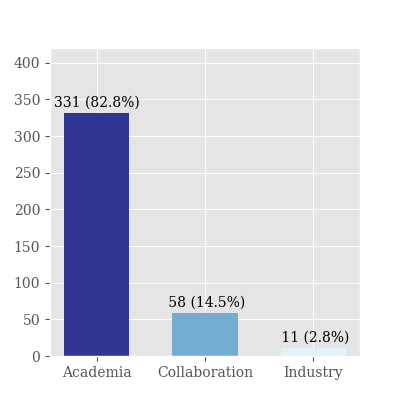
\includegraphics[width=\textwidth]{Affiliation.png}
        \caption{Affiliation}
        \label{fig:affiliation}
    \end{subfigure}
    \begin{subfigure}[b]{0.45\textwidth}
        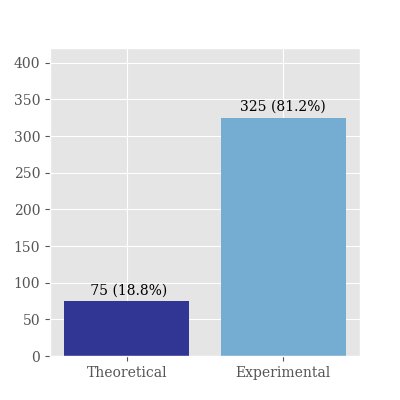
\includegraphics[width=\textwidth]{Research_Type.png}
        \caption{Research type}
        \label{fig:research_type}
    \end{subfigure}
    \begin{subfigure}[b]{0.45\textwidth}
        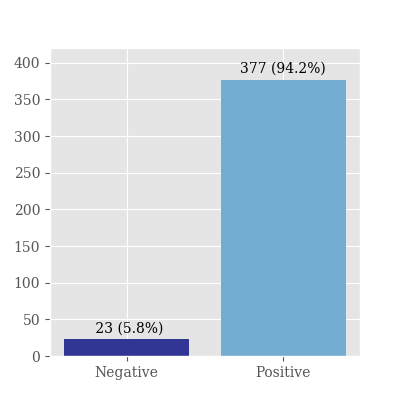
\includegraphics[width=\textwidth]{Result_Outcome.png}
        \caption{Result outcome}
        \label{fig:result_outcome}
    \end{subfigure}
    \begin{subfigure}[b]{0.45\textwidth}
        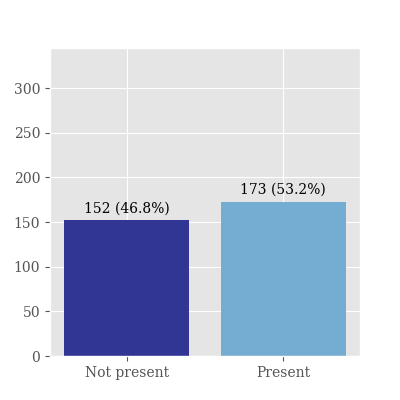
\includegraphics[width=\textwidth]{Third-party_Citation.png}
        \caption{Third-party citations}
        \label{fig:third-party_citation}
    \end{subfigure}
    \caption[Summary of miscellaneous data.]{Summary of miscellaneous data for all 400 papers. Note that for Third-party citation only the 325 experimental papers are relevant, which accounts for the lower values on the left axis.}
    \label{fig:miscellaneous-data}
\end{center}
\end{figure}
\clearpage

\section{Research Transparency}
Research transparency variables describe how well the research method is documented. This includes explicit mentions of: contribution, research goal or objective, hypothesis, prediction, problem description, research method, and research question. The distributions for each variable can be seen in figure~\ref{fig:transparency-data-a} and~\ref{fig:transparency-data-b}.

\begin{figure}[!h]
\begin{center}
    \begin{subfigure}[b]{0.45\textwidth}
        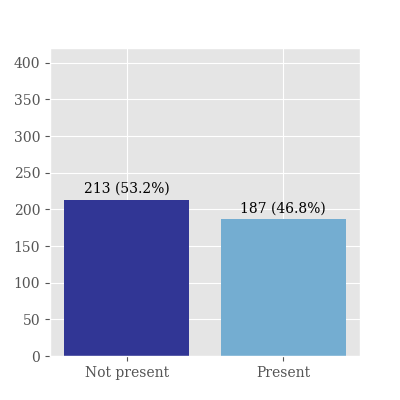
\includegraphics[width=\textwidth]{Contribution.png}
        \caption{Contribution}
        \label{fig:contribution}
    \end{subfigure}
    \begin{subfigure}[b]{0.45\textwidth}
        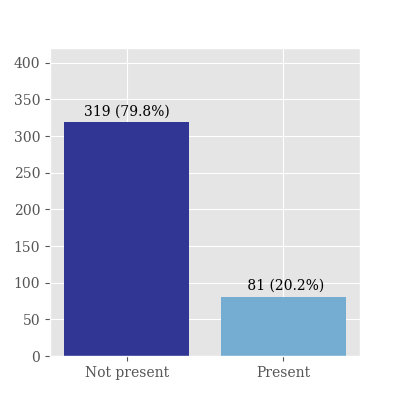
\includegraphics[width=\textwidth]{Goal_or_Objective.png}
        \caption{Goal or objective}
        \label{fig:goal_or_objective}
    \end{subfigure}
    \begin{subfigure}[b]{0.45\textwidth}
        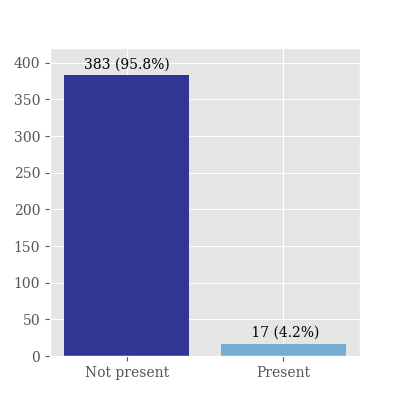
\includegraphics[width=\textwidth]{Hypothesis.png}
        \caption{Hypothesis}
        \label{fig:hypothesis}
    \end{subfigure}
    \begin{subfigure}[b]{0.45\textwidth}
        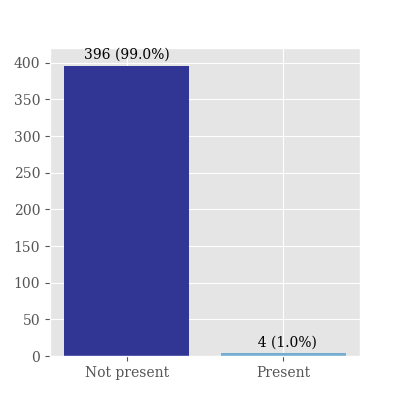
\includegraphics[width=\textwidth]{Prediction.png}
        \caption{Prediction}
        \label{fig:prediction}
    \end{subfigure}
    \caption[Summary of research transparency data.]{Summary of data on research transparency. A term is \emph{Present} if it is explicitly mentioned in a paper. These variables are applicable to all 400 papers.}
    \label{fig:transparency-data-a}
\end{center}
\end{figure}
\begin{figure}[!h]
\begin{center}
    \begin{subfigure}[b]{0.4\textwidth}
        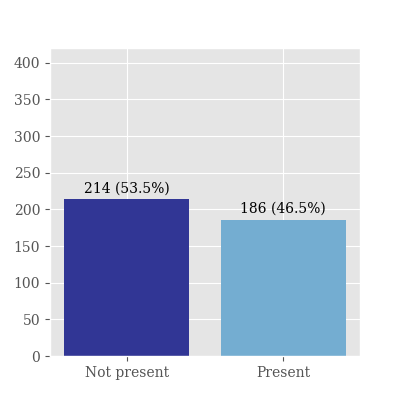
\includegraphics[width=\textwidth]{Problem_Description.png}
        \caption{Problem description}
        \label{fig:problem_description}
    \end{subfigure}
    \begin{subfigure}[b]{0.4\textwidth}
        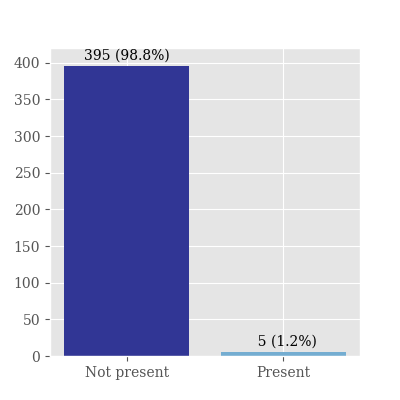
\includegraphics[width=\textwidth]{Research_Method.png}
        \caption{Research method}
        \label{fig:research_method}
    \end{subfigure}
    \begin{subfigure}[b]{0.4\textwidth}
        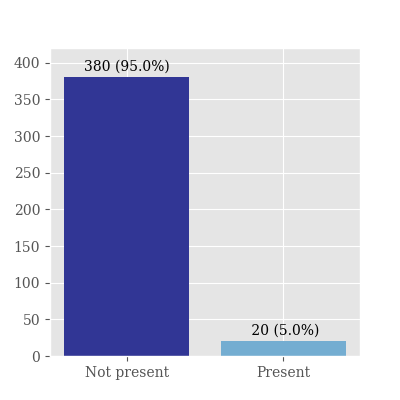
\includegraphics[width=\textwidth]{Research_Question.png}
        \caption{Research question}
        \label{fig:research_question}
    \end{subfigure}
    \caption[Summary of research transparency data continued.]{Continued summary of data on research transparency. A term is \emph{Present} if it is explicitly mentioned in a paper. These variables are applicable to all 400 papers.}
    \label{fig:transparency-data-b}
\end{center}
\end{figure}
\clearpage

\section{Method Documentation}
The method documentation category investigates the availability of the method under investigation through the pseudocode, and open source code variables. Only the 325 experimental papers are relevant for these variables, as seen by the lower values on the left axis compared to the transparency data. The data is summarised in figure~\ref{fig:method_documentation}.

\begin{figure}[!h]
\begin{center}
    \begin{subfigure}[b]{0.4\textwidth}
        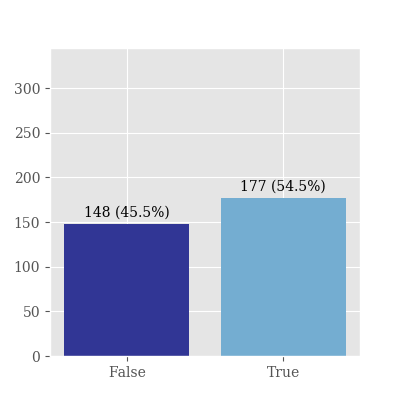
\includegraphics[width=\textwidth]{Pseudocode.png}
        \caption{Pseudocode}
        \label{fig:pseudocode}
    \end{subfigure}
    \begin{subfigure}[b]{0.4\textwidth}
        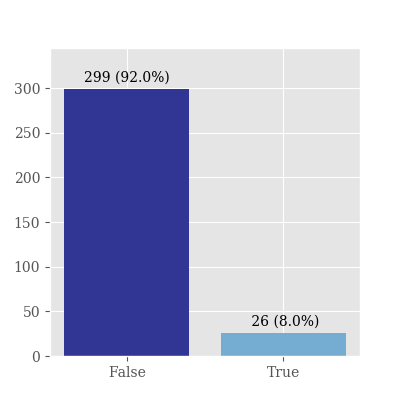
\includegraphics[width=\textwidth]{Open_Source_Code.png}
        \caption{Open source code}
        \label{fig:open_source_code}
    \end{subfigure}
    \caption[Summary of method documentation data.]{Summary of data for the method documentation category. These variables are only applicable to the 325 experimental research papers.}
    \label{fig:method_documentation}
\end{center}
\end{figure}

\section{Experiment Documentation}
Experiment documentation variables relate to how well the experiment is documented and if it is made available. The following variables are included: evaluation criteria, experiment set-up, hardware specification, open experiment code and software dependencies. A summary of the data can be seen in figure~\ref{fig:experiment_documentation}. As in the method documentation category, only the experimental papers are relevant.
\begin{figure}[!h]
\begin{center}
    \begin{subfigure}[b]{0.4\textwidth}
        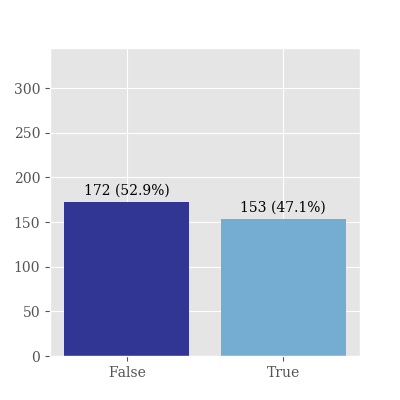
\includegraphics[width=\textwidth]{Evaluation_Criteria.png}
        \caption{Evaluation criteria}
        \label{fig:evaluation_criteria}
    \end{subfigure}
    \begin{subfigure}[b]{0.4\textwidth}
        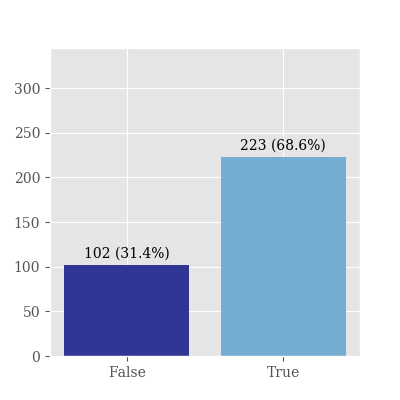
\includegraphics[width=\textwidth]{Experiment_Setup.png}
        \caption{Experiment set-up}
        \label{fig:experiment_setup}
    \end{subfigure}
    \begin{subfigure}[b]{0.4\textwidth}
        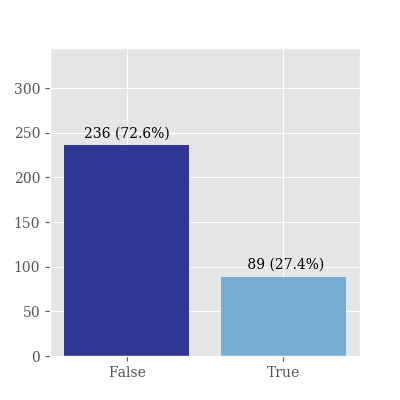
\includegraphics[width=\textwidth]{Hardware_Specification.png}
        \caption{Hardware specification}
        \label{fig:hardware_specification}
    \end{subfigure}
    \begin{subfigure}[b]{0.4\textwidth}
        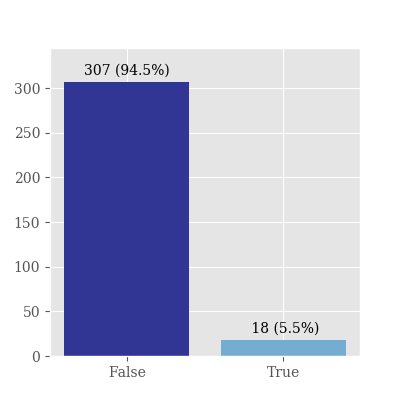
\includegraphics[width=\textwidth]{Open_Experiment_Code.png}
        \caption{Open experiment code}
        \label{fig:open_experiment_code}
    \end{subfigure}
    \begin{subfigure}[b]{0.4\textwidth}
        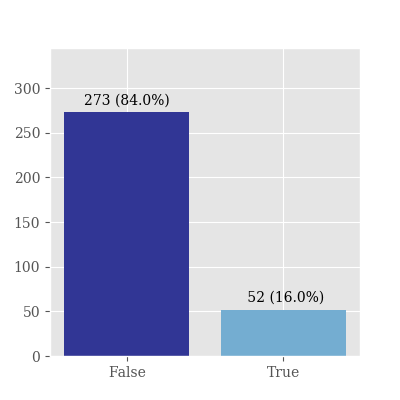
\includegraphics[width=\textwidth]{Software_Dependencies.png}
        \caption{Software dependencies}
        \label{fig:software_dependencies}
    \end{subfigure}
    \caption[Summary of experiment documentation data.]{Summary of data from the experiment documentation category. These variables are only applicable to the 325 experimental research papers.}
    \label{fig:experiment_documentation}
\end{center}
\end{figure}

\section{Open Data}
Open Data relates to the availability of data used during an experiment and documentation of dataset splits. The following variables are included: training data, validation data, test data, and results data. Figure~\ref{fig:open_data} summarizes the results for experimental papers.

\begin{figure}[!h]
\begin{center}
    \begin{subfigure}[b]{0.4\textwidth}
        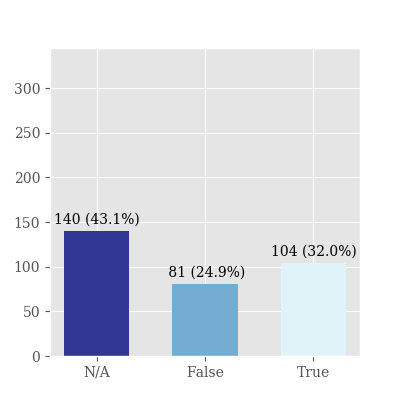
\includegraphics[width=\textwidth]{Training_Data.png}
        \caption{Open training data}
        \label{fig:training}
    \end{subfigure}
    \begin{subfigure}[b]{0.4\textwidth}
        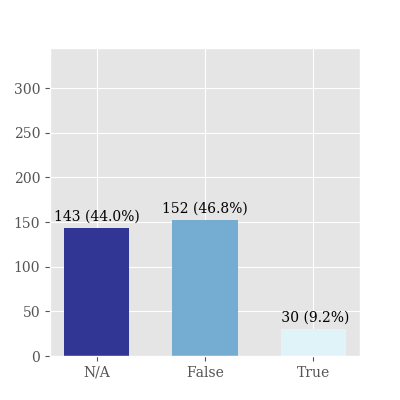
\includegraphics[width=\textwidth]{Validation_Data.png}
        \caption{Open validation data}
        \label{fig:validation}
    \end{subfigure}
    \begin{subfigure}[b]{0.4\textwidth}
        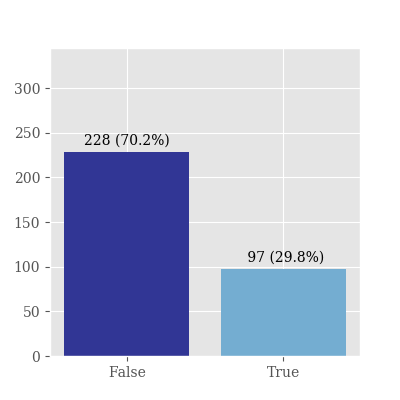
\includegraphics[width=\textwidth]{Test_Data.png}
        \caption{Open test data}
        \label{fig:test}
    \end{subfigure}
    \begin{subfigure}[b]{0.4\textwidth}
        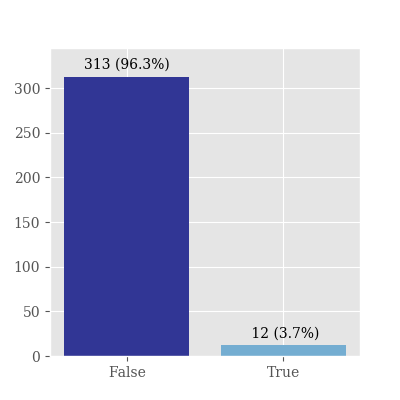
\includegraphics[width=\textwidth]{Results_Data.png}
        \caption{Open results data}
        \label{fig:results}
    \end{subfigure}
    \caption[Summary of the open data category.]{Summary of the open data category. These variables are only applicable to the 325 experimental research papers.}
    \label{fig:open_data}
\end{center}
\end{figure}
\clearpage

\section{Researcher Error}
\label{sec:researcher_error}
The data for Third-party citations and Result outcome have been excluded from further analysis due to inaccurate data and researcher error, respectively.

For Third-party citations, the intent was to record citations of software and data used for an experiment. This intent was to investigate if public datasets and published source code is cited when used by other researchers. For the most part, the papers noted with \emph{Present} in figure~\ref{fig:third-party_citation} show correct citations to public datasets. However, it is difficult to say what portion of the \emph{Not present} papers have used public datasets or source code, or only mentioned them by name without a correct citation.

Result outcome (figure~\ref{fig:result_outcome}) was erroneously recorded as a positive result, instead of a notion of the novelty of the research. This would be any paper that presents confirmation of a hypothesis, or where the wording of their findings present a solution or improvement to something. Since very few papers include a hypothesis in the first place, the data for this variable is excluded from any further analysis.

\section{Patterns of Analysis Revisited}
Author affiliation

Conference view on supplemental material

Changes over time

\cleardoublepage
